%!TEX root = Projeto.tex
\subsection{Conceitos básicos}

\subsubsection{Segurança da informação}
O glossário do padrão ISO/IEC 27000 \cite{ISO2016} define segurança da informação como um processo cujos objetivos são a ``preservação da confidencialidade, integridade e disponibilidade da informação''. \citeinline{Foster1998} elabora esses objetivos, descrevendo a confidencialidade como a condição na qual a informação só pode ser acessada pelos agentes autorizados, integridade como a capacidade de proteger a informação contra modificações não autorizadas, e a disponibilidade como a capacidade de garantir acesso à informação quando necessário; \citeinline{Foster1998} ainda atribui mais duas características a um sistema de segurança da informação: \poe{accountability} como a possibilidade de se atribuir um agente para cada ação ocorrida dentro do sistema, e \poe{assurance} como o grau de confiabilidade na segurança do sistema em relação aos seus objetivos declarados. Esses cinco parâmetros -- confidencialidade, integridade, disponibilidade, \poe{accountability} e \poe{assurance} -- representam aspectos da qualidade de uma estratégia para a segurança da informação, e servirão como base para a avaliação das soluções sob consideração neste trabalho.

Um sistema de informação complexo como a web é produto da colaboração de múltiplos participantes, todos co-responsáveis pela segurança da informação que trafega entre eles. Porém, para a delimitação de escopo deste trabalho, qualquer definição de segurança da informação será restrita aos sistemas envolvidos nas atividades de navegação que os usuários exercem através da web. Isso inclui os seguintes participantes: provedores de serviço (\poe{sites}, servidores da web), protocolos de comunicação em rede (HTTP, HTTPS, \poe{web sockets}), o software navegador e o ambiente de execução de Javascript a ele incorporado. Isto delimita a área de conhecimento relevante para este trabalho, ilustrado pelo diagrama \ref{Fig: diagrama04}.

\begin{figure}[h]
	\centering
	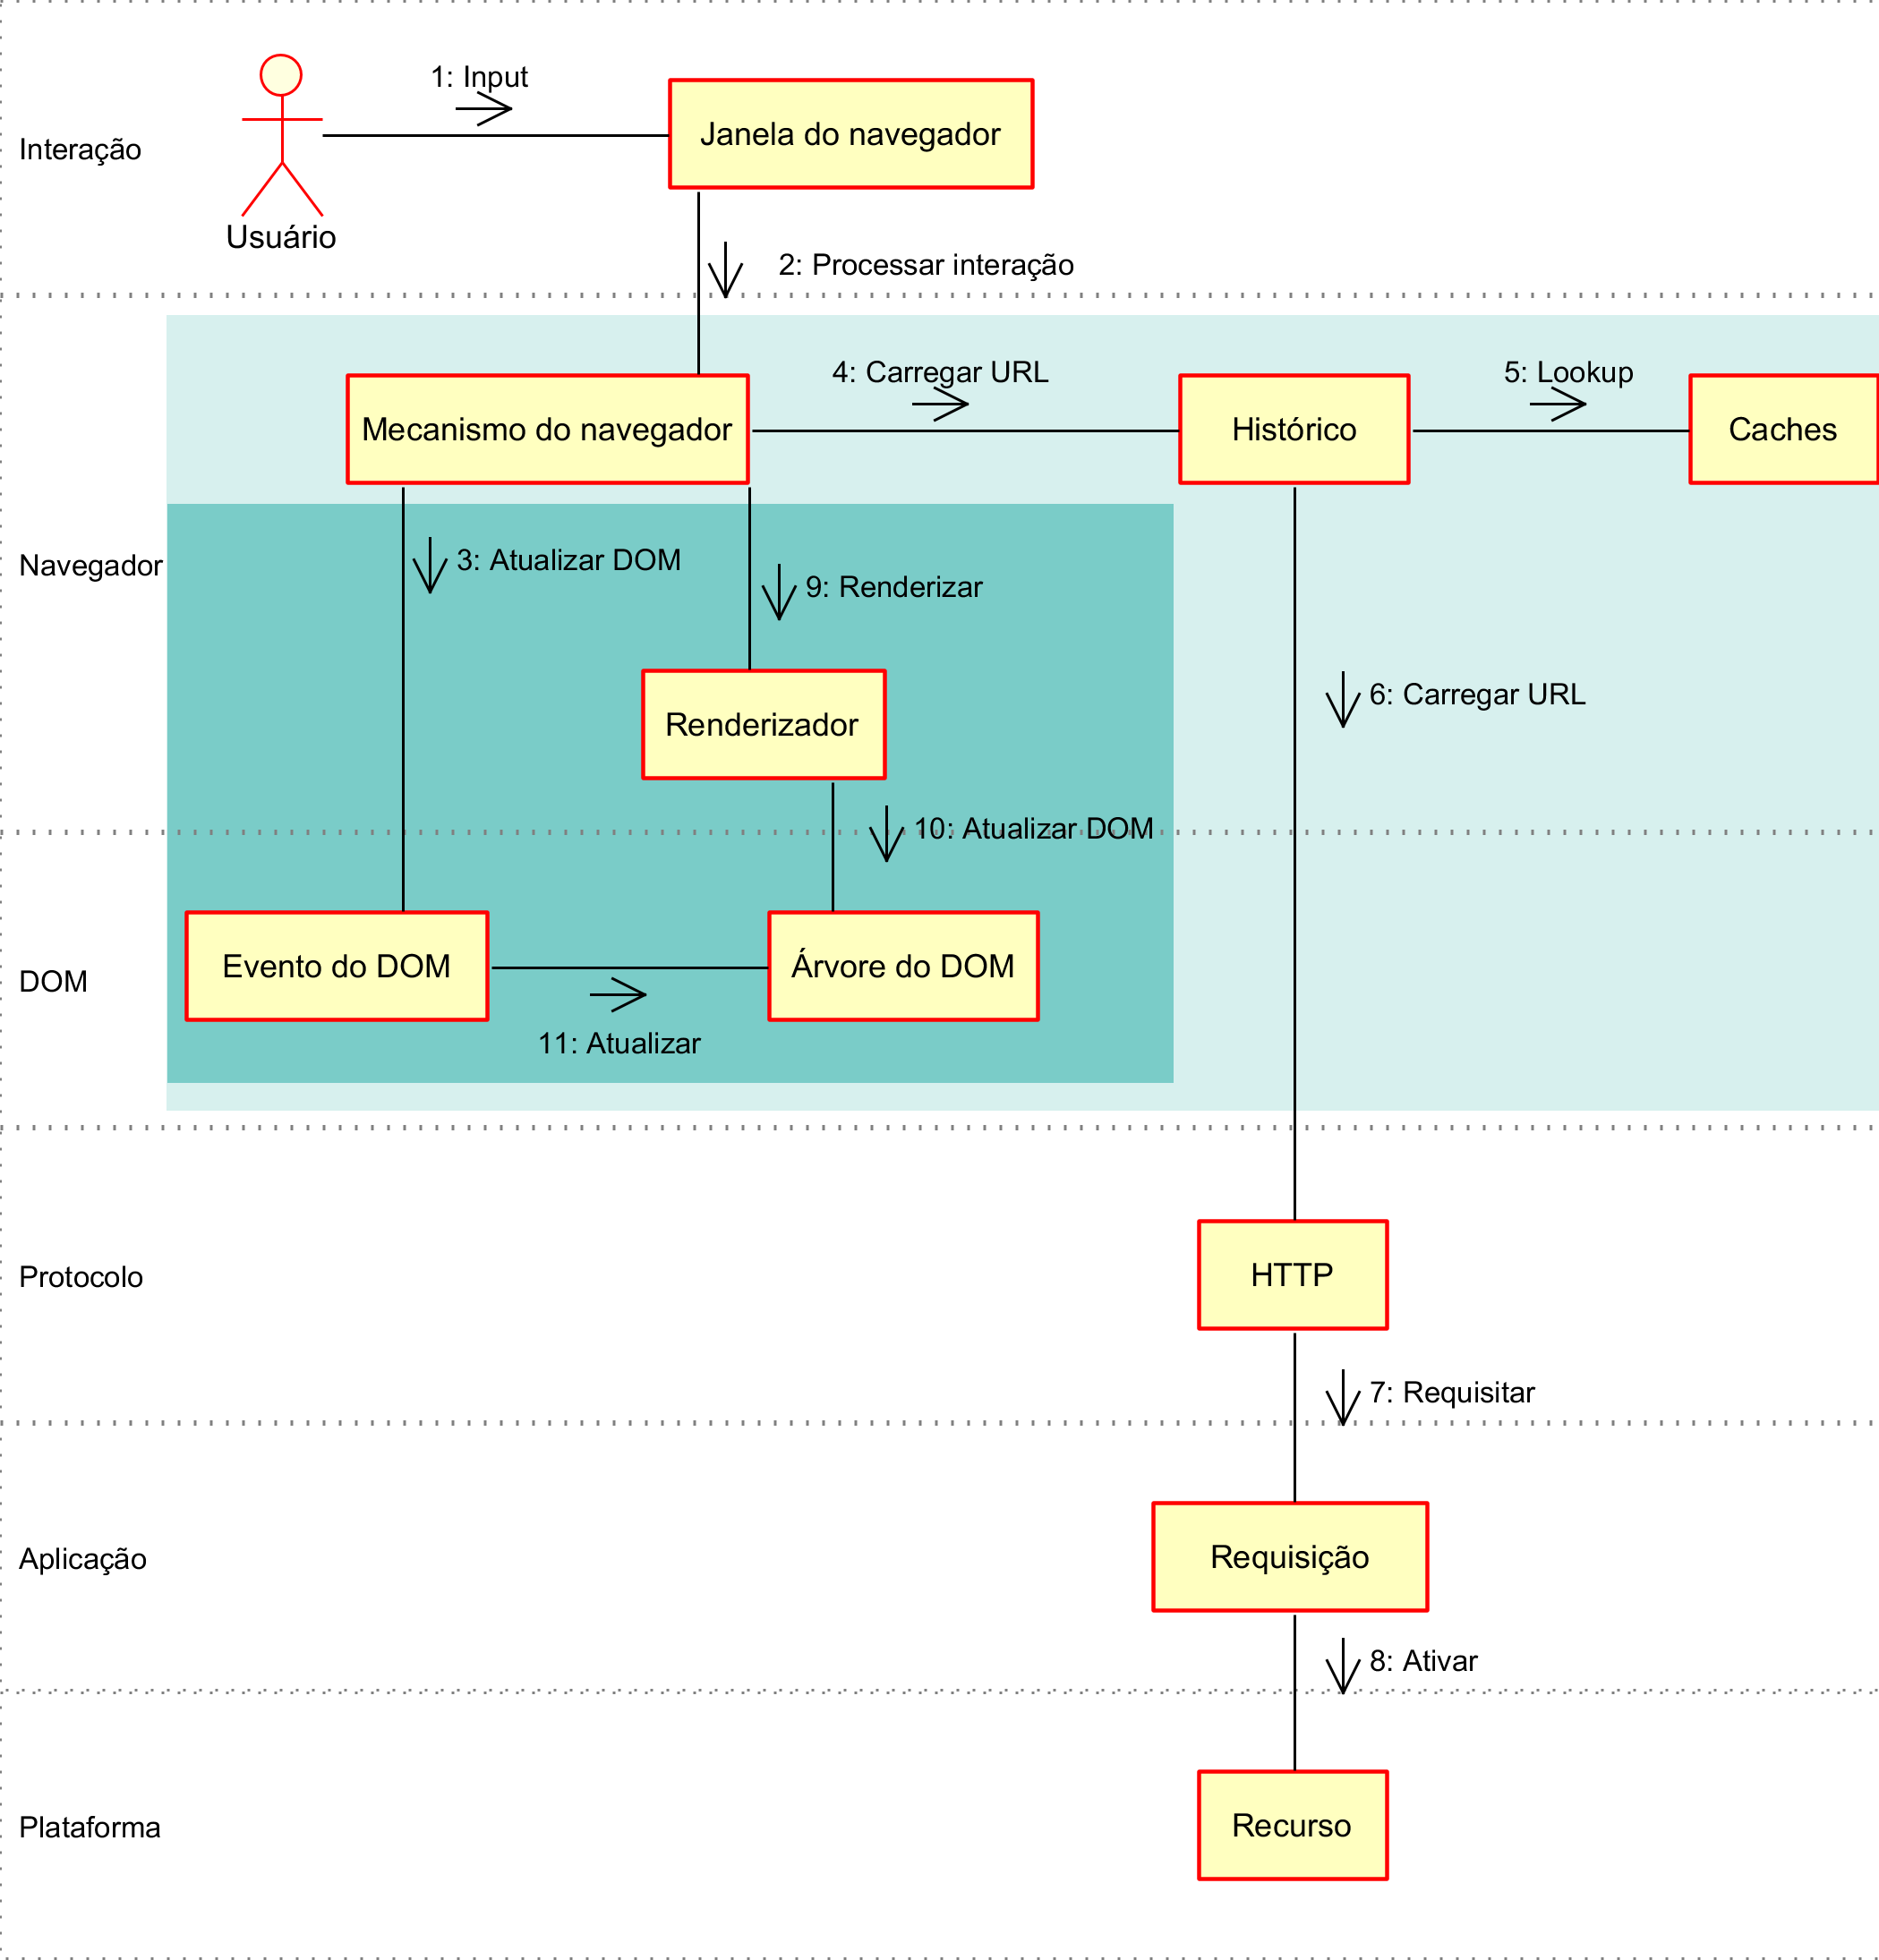
\includegraphics[width=12cm]{diagramas/escopo.png}
	\label{Fig: diagrama04}
	\caption[Sistema de informação em contexto de aplicação web]
	{Sistema de informação em contexto de aplicação web. A área sinalizada em azul corresponde ao escopo do estado da arte em segurança da informação em aplicações web, e a sub-área em azul intenso compreende o escopo da proposta descrita na seção 3 deste trabalho.}
\end{figure}

%\subsection{Políticas de controle de acesso}
%Segundo \cite{Goguen1982}, uma política de controle de acesso é necessária para que se estabeleçam quais fluxos de dados serão permitidos em um sistema de informação.

\subsubsection{Modelos de controle de acesso}
O trabalho seminal de \citeinline{Goguen1982} estabelece distinção entre as ``políticas de segurança'' e os ``modelos de segurança'' para evidenciar aspectos complementares da segurança da informação em sistemas de software. Segundo \citeauthor{Goguen1982}, uma \poe{política de segurança} define os requisitos de segurança da informação para um dado sistema, enquanto um ``modelo de segurança'' é a especificação da forma como esse sistema irá implementar uma política de segurança. Categorizando modelos de segurança, \citeinline{Foster1998} os divide entre ``discricionários'', sob a sigla DAC (DAC -- \poe{discretionary access control}), e ``mandatórios'', sob a sigla MAC (MAC -- \poe{mandatory access control}). Essas duas categorias nascem de abordagens opostas, com implicações fundamentais sobre a natureza das soluções de apoio à segurança da informação.

Para \citeauthor{Foster1998} o conceito central dos modelos discricionários é a segurança observada no relacionamento entre agentes e objetos em um sistema. Por exemplo, quando uma política estabelece que um {\script} -- a parte ``agente'' -- não pode iniciar conexões com domínios diferentes do seu próprio -- a parte ``objeto'', um modelo DAC bem sucedido impedirá que a parte ``relacionamento'', representada pelas conexões de rede, possa acontecer. Modelos discricionários são os mais comumente utilizados para estabelecer mecanismos de segurança nos navegadores. Do ponto de vista da segurança da informação, modelos de DACs não podem garanti-la  fora do contexto dos relacionamentos pré-estabelecidos pelas políticas. Isto significa, por exemplo, que dados legitimamente obtidos dentro de regras discricionárias pode ser replicado para um contexto não-seguro sem qualquer impedimento derivado do modelo de segurança.

Sobre os modelos mandatórios, \citeauthor{Foster1998} caracteriza-os pela existência de níveis de confidencialidade que classificam os participantes do sistema de informação, viabilizando o controle dinâmico do trânsito da informação entre os agentes. Num modelo mandatório, o nível de segurança de um objeto de informação -- seja ele um arquivo, um registro de dados, um valor numérico ou qualquer outro dado -- impede que ele seja obtido ou modificado por agentes aos quais tenham sido atribuídos níveis de segurança mais baixos. Modelos baseados em MAC exercem segurança em âmbito sistêmico, atuando sobre todas as trocas de informação, o que contrasta com a aplicação localizada das regras de segurança observadas em modelos baseados em DAC. Por causa dessa característica, \citeauthor{Foster1998} sugere que o controle do fluxo da informação faz dos MACs modelos mais robustos do que os DACs.

\subsubsection{Controle do fluxo de informações}
O controle do fluxo de informações (IFC -- \poe{information flow control}) é um mecanismo que atua, em tempo de execução, nos meios de propagação dos valores entre os espaços de armazenamento de um sistema computacional de modo a impedir fluxos não autorizados dos dados \cite{Denning1976}. IFC implementa um modelo de controle de acesso do tipo mandatório e baseia-se em \poe{classes de segurança} ``altas'' e ``baixas'', simbolizadas pelas letras \html{<h>} e \html{<l>}, respectivamente, para indicar graus de confidencialidade das informações e dos seus espaços de armazenamento (\poe{heap}, pilha, redes, dispositivos etc). Operações entre entidades com classes de segurança diferentes, como a cópia do valor de uma variável \html{<h>} (confidencial) para a variável \html{<l>} (pública), são automaticamente impedidas de acontecerem, ocasionando falha de execução.

IFC distingue entre fluxos de informação ``explícitos'' e ``implícitos''. Um fluxo explícito ocorre quando uma informação classificada como ``alta'' é diretamente copiada para um contexto de classificação ``baixa'', como na listagem de código \ref{Src: jsIFCExplicitFlow}. Em um fluxo implícito, não é a informação em si que transita entre contextos de classificação diferente, mas sim alguma informação derivada dela através da qual seja possível fazer qualquer inferência sobre seu conteúdo. Um exemplo de fluxo implícito encontra-se la listagem \ref{Src: jsIFCImplicitFlow}. Um mecanismo que suporte IFC deve ser capaz de interromper vazamento de informação em ambos os tipos de fluxo.

\lstinputlisting[language=JavaScript,
inputencoding=utf8,
label={Src: jsIFCExplicitFlow},
caption={Vazamento de dados em fluxo explícito de informação}]{codigo/sample02-ifc-implicit.js}

\lstinputlisting[language=JavaScript,
inputencoding=utf8,
label={Src: jsIFCImplicitFlow},
caption={Vazamento de dados em fluxo implícito de informação}]{codigo/sample03-ifc-explicit.js}